%----------------------------------------------------------------------------------------
%	PACKAGES AND OTHER DOCUMENT CONFIGURATIONS
%----------------------------------------------------------------------------------------
\documentclass[13pt]{scrartcl} % Font size
% \documentclass[12pt]{article} % Font size
%----------------------------------------------------------------------------------------
%	PACKAGES AND OTHER DOCUMENT CONFIGURATIONS
%----------------------------------------------------------------------------------------

\usepackage{amsmath, amsfonts, amsthm} % Math packages

% Packages for Title Page
\usepackage{newlfont}
\usepackage{gensymb}

\usepackage{listings} % Code listings, with syntax highlighting

\usepackage[utf8]{inputenc}
% \usepackage[english,vietnam]{babel}
% \usepackage[utf7]{vietnam}

%----------------------------------------------------------------------------------------
%	IMAGES CONFIGURATION
%----------------------------------------------------------------------------------------
\usepackage{graphicx} % Required for inserting images
\graphicspath{{Figures/}{./}} % Specifies where to look for included images (trailing slash required)
\usepackage{xstring}

\usepackage{subcaption}
\DeclareCaptionFormat{custom}
{
	\normalsize{\bf#1}\textbf{#2}\textit{\small #3}
}
\captionsetup{format=custom}


%----------------------------------------------------------------------------------------
%	LIST CONFIGURATION
%----------------------------------------------------------------------------------------
\usepackage{enumitem} % Required for list customisation
\setlist{noitemsep} % No spacing between list items


%----------------------------------------------------------------------------------------
%	PARAGRAPH FORMATTING 
%----------------------------------------------------------------------------------------
% \setlength\parindent{0pt} % Removes all indentation from paragraphs
% \setlength{\parindent}{2em}
\usepackage{indentfirst}
\usepackage[skip=10pt plus1pt, indent=25pt]{parskip}

%----------------------------------------------------------------------------------------
%	DOCUMENT MARGINS
%----------------------------------------------------------------------------------------
\usepackage{geometry} % Required for adjusting page dimensions and margins

\geometry{
	paper=a4paper, % Paper size, change to letterpaper for US letter size
	top=2cm, % Top margin
	bottom=2.5cm, % Bottom margin
	left=3cm, % Left margin
	right=3cm, % Right margin
	headheight=0.75cm, % Header height
	footskip=1.5cm, % Space from the bottom margin to the baseline of the footer
	headsep=0.75cm, % Space from the top margin to the baseline of the header
	%showframe, % Uncomment to show how the type block is set on the page
}

%----------------------------------------------------------------------------------------
%	FONTS
%----------------------------------------------------------------------------------------
% \usepackage[utf8]{inputenc} % Required for inputting international characters
% \usepackage[T1]{fontenc} % Use 8-bit encoding
\usepackage{fourier} % Use the Adobe Utopia font for the document

%----------------------------------------------------------------------------------------
%	SECTION 
%----------------------------------------------------------------------------------------
% \setcounter{section}{14}
% \usepackage{sectsty} % Allows customising section commands

% \sectionfont{\vspace{6pt}\centering\normalfont\scshape} % \section{} styling
% \subsectionfont{\normalfont\bfseries} % \subsection{} styling
% \subsubsectionfont{\normalfont\itshape} % \subsubsection{} styling
% \paragraphfont{\normalfont\scshape} % \paragraph{} styling

%----------------------------------------------------------------------------------------
%	HEADERS AND FOOTERS
%----------------------------------------------------------------------------------------

\usepackage{scrlayer-scrpage} % Required for customising headers and footers

\ohead*{} % Right header
\ihead*{} % Left header
\chead*{} % Centre header

\ofoot*{} % Right footer
\ifoot*{} % Left footer
\cfoot*{\pagemark} % Centre footer
 % Include the file specifying the document structure and custom commands
\usepackage[utf8]{vietnam}

\title{Chương 15: Các hệ thống trực quan hóa}
%!TEX encoding = UTF-8 Unicode
\textwidth=450pt\oddsidemargin=5pt
\begin{document}

%----------------------------------------------------------------------------------------
%	TITLE PAGE
%----------------------------------------------------------------------------------------
\begin{titlepage}
    \begin{center}
        {{\Large{\textsc{TRƯỜNG ĐẠI HỌC KHOA HỌC TỰ NHIÊN \\ ĐẠI HỌC QUỐC GIA HÀ NỘI}}}} \rule[0.1cm]{15.8cm}{0.1mm}
        \rule[0.5cm]{15.8cm}{0.6mm}
        {\large{\bf KHOA TOÁN - CƠ - TIN HỌC \\ CHUYÊN NGÀNH KHOA HỌC DỮ LIỆU }}
    \end{center}

    % \vspace{5mm}

    \begin{figure}[!ht] % [!ht] forces the figure to be output where it is defined in the code (it suppresses floating)
        \centering
        
\includegraphics[width=0.25\columnwidth]{hus.jpeg}
    \end{figure}

    % \vspace{5mm}

    \begin{center}
        {\LARGE{\bf CHƯƠNG 15: VISUALIZATION SYSTEMS \\ CÁC HỆ THỐNG TRỰC QUAN HÓA}}
    \end{center}

    \vspace{5mm}


    \begin{center}
        \large{Môn học: Trực quan hóa dữ liệu}
    \end{center}

    %    \begin{center}
    % 	{\fontsize{14pt}{1}\selectfont Ngành: Khoa học dữ liệu}
    % \end{center}
    \vspace{25mm}

    \hspace{0cm}\begin{minipage}[t]{0.7\textwidth}
        \normalsize{GIẢNG VIÊN:} \\
        \-\hspace{1cm}\large\textbf{TS. Nguyễn Thị Bích Thủy}
    \end{minipage}
    \par
    \vspace{5mm}

    \hspace{0cm}\begin{minipage}[t]{0.7\textwidth}
        \normalsize
        HỌC VIÊN: \\
        \-\hspace{1cm}\large\textbf{Vũ Minh Hưng} \\
        \-\hspace{1cm}\large\textbf{Vũ Trang Linh}
    \end{minipage}
    \par
    \vfill
    \begin{center}
        {\large{\bf Tháng 12 năm 2022 }}
    \end{center}
\end{titlepage}


%----------------------------------------------------------------------------------------
%	TABLE OF CONTENTS
%----------------------------------------------------------------------------------------

% \renewcommand*\contentsname{Summary}
\date{ }
% \maketitle
\tableofcontents

\pagebreak
% \newpage
%----------------------------------------------------------------------------------------
%	INTRODUCTION
%----------------------------------------------------------------------------------------

\section{Lời giới thiệu}
Trong chương này chúng tôi giới thiệu qua một số hệ thống và công cụ trực quan hóa thông tin và dữ liệu. Chúng tôi tập trung ưu tiên các phần mềm miễn phí, cho phép học viên quan tâm tìm hiểu sâu hơn về lĩnh vực trực quan hóa có thể thử nghiệm các công cụ này. Đây chỉ là một số trong rất nhiều các công cụ rất tốt để trực quan hóa dữ liệu mà không được để cập tới trong chương này, bạn độc có thể tự tìm kiếm và tải chúng về dùng thử. Chúng tôi cũng đề cập tới một số công cụ có trả phí mà có các chức năng tương đương với các hệ thống chúng tôi đề cập tới. Lưu ý rằng các đường link của các công cụ là chính xác tại thời điểm xuất bản cuốn sách này, nhưng có thể thay đổi sau này, và một số công cụ có thể không còn được phát hành miễn phí nữa.

%----------------------------------------------------------------------------------------
%	SECTION 1
%----------------------------------------------------------------------------------------

\section{Các hệ thống dựa trên loại dữ liệu}

\subsection{Dữ liệu khoa học}

OpenDX, ban đầu được giới thiệu là một Công cụ khai phá dữ liệu trực quan hóa của IBM, là một môi trường trực quan hóa ban đầu được sử dụng cho phân tích dữ liệu kỹ thuật và khoa học. Cái tách biệt công cụ này với các nền tảng trực quan hóa khá là tiến trình quy hoạch trực quan được sử dụng để tùy biến trực quan hóa. Chức năng Network Editor cho phép người dùng kéo thả các thành phần vào một giao diện và tạo các đường liên kết giữa các thành phần này để biểu diễn sự tương tác dữ liệu tương ứng. Các thành phần thường được xếp vào một vài lớp đối tượng, bao gồm:
\begin{itemize}
    \item Nhập và xuất – các mô đun sử dụng để tải và lưu dữ liệu trong các định dạng khác nhau;
    \item Điều hướng xử lý – các mô đun để tạo các vòng lặp và thực thi theo điều kiện;
    \item Hiện thực hóa – các mô đun để ánh xạ dự liệu vào các thực thể có thể hiển thị, ví dụ như các đẳng diện, lưới, hoặc các đường hướng.
    \item Hiển thị – các mô đun điều khiển các thuộc tính hiển thị, như ánh sáng, góc quay, cắt xén.
    \item Biến đổi – các chức năng áp dụng cho dữ liệu, ví dụ như lọc, các hàm toán học, sắp xếp;
    \item Tương tác – các mô dun như là trình chọn tệp, menu, dial/slider, và các nút bấm.
\end{itemize}

\begin{figure}[!ht] % [!ht] forces the figure to be output where it is defined in the code (it suppresses floating)
    \centering
    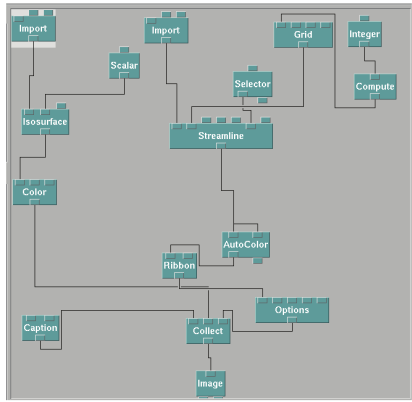
\includegraphics[width=0.7\columnwidth]{1.png}
    \caption{Ví dụ về một mạng lưới trong OpenDX. Luồng xử lý bắt đầu từ mô đun Import tới đầu ra Image.}
\end{figure}

\begin{figure}[!ht] % [!ht] forces the figure to be output where it is defined in the code (it suppresses floating)
    \centering
    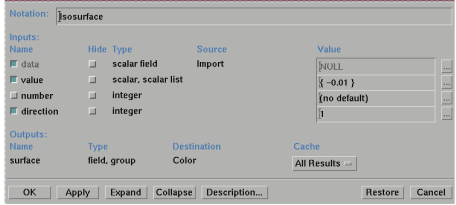
\includegraphics[width=0.8\columnwidth]{2.png}
    \caption{Một ví dụ về giao diện của một mô đun trong OpenDX. Một số tham số cần tự thiết lập, trong khi số khác được thiết lập bằng cách kết nối một tab input hoặc output của một mô đun tới input hoặc output của mô đun khác.}
\end{figure}

\begin{figure}[!ht] % [!ht] forces the figure to be output where it is defined in the code (it suppresses floating)
    \centering
    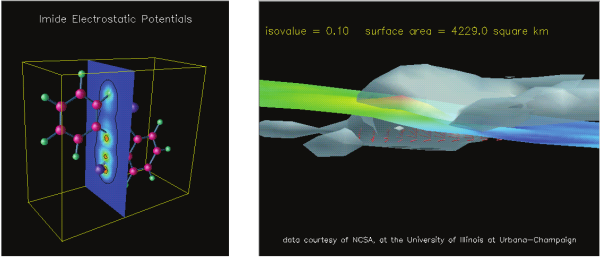
\includegraphics[width=0.7\columnwidth]{3.png}
    \caption{Các ví dụ về trực quan hóa có thể được tạo với OpenDX. Hình đầu kết hợp một mặt cắt qua một trường điện từ, trong khi ở hình thứ 2 kết hợp nhiệt độ, độ ẩm và vùng gió để xem xét các thuộc tính của một đám mây bão.}
\end{figure}

%------------------------------------------------
\newpage
\subsection{Dữ liệu đa biến}

XmdvTool, phát triển bởi Matthew Ward, Elke Rundensteiner và các cộng sự ở Viện Bách Khoa Worcester, là một gói phần mềm trực quan hóa tích hợp năm phương pháp chung cho trực quan hóa dữ liệu đa biến trong một ứng dụng duy nhất. Bộ công cụ này bao gồm ma trận biểu đồ phân tán, biểu đồ phần tán hình sao, các tọa độ song song, xếp chồng theo chiều, và các phương pháp hướng pixel. Các phương pháp trực quan hóa này được liên kết với nhau sử dụng một cơ chế chọn lọc đơn giản gọi là N-dimensional brush, bằng cách định nghĩa một siêu hộp trong không gian dữ liệu. Dữ liệu được lựa chọn trong một view cũng sẽ được chọn trong view khác, và kết quả lựa chọn sẽ được bôi đậm, đánh dấu, xóa đi hoặc phân tích tách rời khỏi toàn bộ dữ liệu.

Ngoài mục tiêu ban đầu, XmdvTool còn được mở rộng để bao gồm thêm các tính năng kiến trúc để hỗ trợ các tập dữ liệu lớn. Ban đầu, Ying Huey Fua giới thiệu hệ tọa độ song song phân cấp cho khai phá dữ liệu có chứa nhiều ghi chép. Dữ liệu được phân cụm theo cấp và kết quả được hiển thị trong một hệ tọa độ song song sử dụng độ trong suốt là biến số. Sau đó công cụ được thêm brush dựa trên cấu trúc, là một giao diện người dùng tích hợp cho duyệt và vẽ bên trong cấu trúc dữ liệu phân cấp. Jing Yang sau đố tổng quát hóa ứng dụng của cấu trúc dữ liệu phân cấp này với các công cụ trực quan hóa khác của XmdvTool và định nghĩa ra framework hiển thị phân cấp tương tác. Thêm vào đó, XmdvTool cung cấp một framework giảm chiều phân cấp trực quan mà có thể nhóm lại và tổ chức không gian các chiều, cung cấp các không gian con có ý nghĩa cho việc phân tích. XmdvTool cũng bao gồm cách tiếp cận phân lớp số lượng theo khoảng cách để xử lý các biến danh nghĩa và các công cụ để sắp xếp lại các chiều để giảm sự lộn xộn trực quan.

\begin{figure}[!ht] % [!ht] forces the figure to be output where it is defined in the code (it suppresses floating)
    \centering
    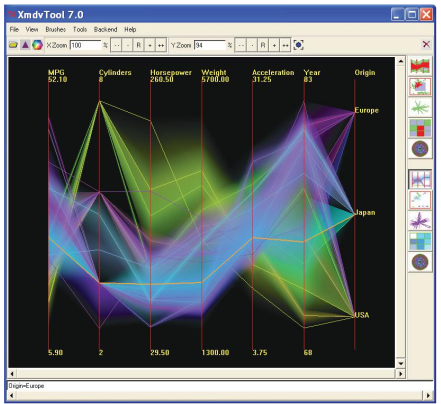
\includegraphics[width=0.8\columnwidth]{4.png}
    \caption{Ví dụ về hệ tọa độ song song phân cấp trong XmdvTool. Mỗi đường mảnh đại diện cho tâm của một nhóm, và dải mờ quanh mỗi đường trung tâm chỉ phạm vi của nhóm trong mỗi chiều. Vùng mờ gần tâm để chỉ dân số của mỗi nhóm. }
\end{figure}


XmdvTool được giới thiệu lần đầu vào năm 1994, và tại thời điểm viết cuốn sách này, nó ở phiên bản 7.0. Ngoài định dạng file của ứng dụng, nó có thể hỗ trợ bảng biểu Excel hoặc cơ sở dữ liệu Oracle. Ứng dụng này được ứng dụng rộng rãi trong các ứng dụng như khoa học không gian và trái đất, sinh tin học, nghiên cứu dân số và phân tích hiệu năng của mạng lưới.

\begin{figure}[!ht] % [!ht] forces the figure to be output where it is defined in the code (it suppresses floating)
    \centering
    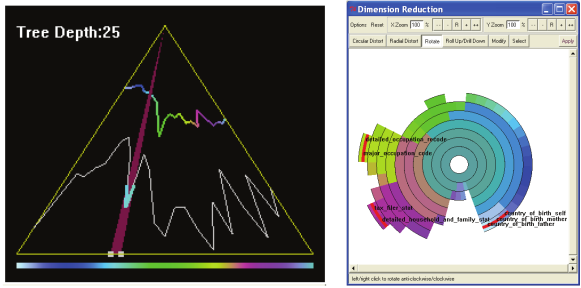
\includegraphics[width=0.8\columnwidth]{5.png}
    \caption{Hiển thị các cấu trúc phân cấp trong XmdvTool. Hình đầu là brush dựa trên cấu trúc sử dụng để điều hướng và lựa chọn trong một phân cấp dữ liệu. Hình thứ hai là InterRing, cho phép người dùng phân loại các chiều dữ liệu và lựa chọn tập con hoặc trung bình các chiều cho hiển thị dữ liệu.}
\end{figure}

Một số phần mềm có chức năng tương tự với XmdvTool bao gồm Spotfire, và Tableau (có trả phí), các phần mềm này đều có nhiều chức năng hơn XmdvTool.

%------------------------------------------------

\subsection{Dữ liệu đồ thị}

GraphViz là một thư viện các thuật toán dựa trên đồ thị phát triển ở Viện Nghiên cứu ATT. Kiến trúc và triết lý của GraphViz là khá độc nhất khi so sánh với các công cụ trực quan hóa khác. Nó hỗ trợ một loạt các phương pháp chuyên cho đồ thị, các phương pháp trình bày và các phương pháp hiển thị. Tong khi một số thành phần tương tác đã được tích hợp trong hệ thống, phần mềm này chủ yếu vẫn thiên về dòng lệnh. Người dùng lựa chọn một tệp mô tả đồ thị và truyền vào mô đun trình bay, cùng với định dạng đầu ra mong muốn. Định dạng đầu ra được hỗ trợ rất nhiều và dễ dàng ích hợp các kết quả vào các tài liệu, website và ứng dụng.

Tất cả các chương trình GraphViz yêu cầu tệp truyền vào ở dạng ngôn ngữ DOT, bên dưới là một ví dụ của đồ thị định nghĩa trong ngôn ngữ DOT:

\begin{figure}[!ht] % [!ht] forces the figure to be output where it is defined in the code (it suppresses floating)
    \centering
    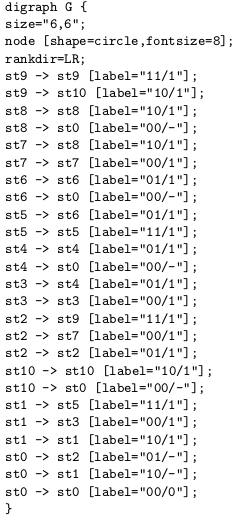
\includegraphics[width=0.45\columnwidth]{6.png}
\end{figure}

Mỗi dòng định nghĩa các thuộc tính của một đồ thị gồm các đỉnh, các cạnh. Cả đồ thị vô hướng và có hướng đều được hỗ trợ. Hình 15.6 bên dưới sử dụng bốn kiểu trình bày đồ thị, bao gồm:
\begin{itemize}
    \item Dot – tiếp cận theo lớp, độ thị có các cạnh theo cùng một hướng.
    \item Neato – mô hình dựa trên mở rộng đa chiều
    \item Circos – trình bày theo vòng tròn, thương hiệu quả cho các mạng thông tin.
    \item Fdp – phương pháp hướng lực sử dụng phỏng đoán đa lưới, cho phép biểu diễn được các đồ thị rất lớn.
\end{itemize}

\begin{figure}[!ht] % [!ht] forces the figure to be output where it is defined in the code (it suppresses floating)
    \centering
    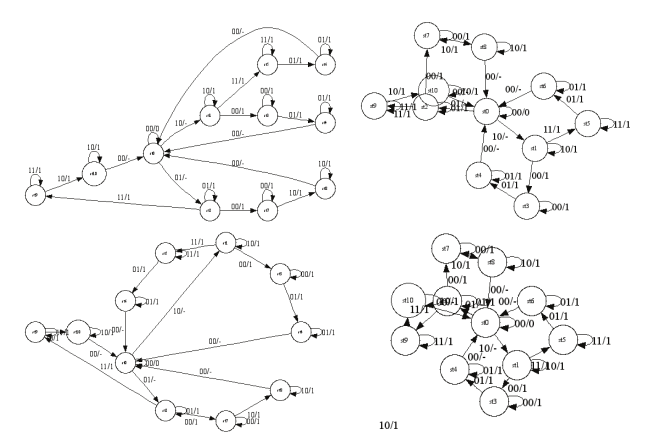
\includegraphics[width=0.8\columnwidth]{7.png}
    \caption{Đầu ra của GraphViz, đại diện cho một đồ thị với 4 cách trình bày khác nhau.}
\end{figure}

Công cụ khác cũng sử dụng để biểu diễn đồ thị là Tom Sawyer Sofware (có mất phí).


%----------------------------------------------------------------------------------------
%	SECTION 2
%----------------------------------------------------------------------------------------
\section{Các hệ thống dựa trên loại phân tích}
\subsection{Thống kê}
GGobi là một công cụ tương tác cho phân tích và trực quan hóa dữ liệu đa biến phát triển bởi Deborah Swayne, Dianne Cook và Andreas Buja vào đầu những năm 1990 tại Bellcore, Inc. Nó hỗ trợ một số phương pháp trực quan hóa, bao gồm biểu đồ phân tán, ma trận biểu đồ phân tán, biểu đồ cột, đồ thị và các tọa độ song song (xem hình 15.7).

\begin{figure}[!ht] % [!ht] forces the figure to be output where it is defined in the code (it suppresses floating)
    \centering
    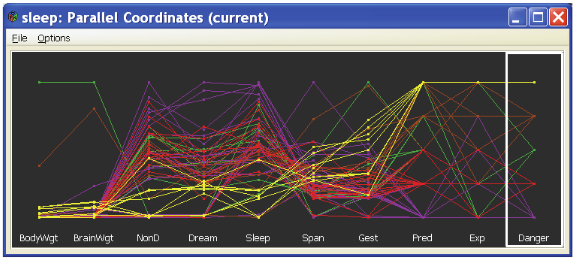
\includegraphics[width=0.8\columnwidth]{8.png}
    \caption{Ví dụ về các tọa độ song song trong ứng dụng GGobi.}
\end{figure}

Với mỗi phương pháp trực quan hóa, bản điều khiển tương ứng sẽ được hiển thị bằng cách ấn vào phương pháp đó. Màu sắc được sử dụng để liên kết dữ liệu giữa nhiều phần hiển thị, và người dùng sẽ có nhiều tùy chọ để điều chỉnh màu sắc tương ứng với mỗi thực thể đồ họa. Người dùng bắt đầu bằng việc lựa chọn một chiều dữ liệu để điều chỉnh màu sắc, một biểu đồ histogram có thể được sử dụng để điều chỉnh khoảng giá trị gán với mỗi màu (hình 15.8). Bôi màu được liện kết có thể được sử dụng để bôi đậm một điểm dữ liệu được lựa chọn ở mỗi màn hình.

\begin{figure}[!ht] % [!ht] forces the figure to be output where it is defined in the code (it suppresses floating)
    \centering
    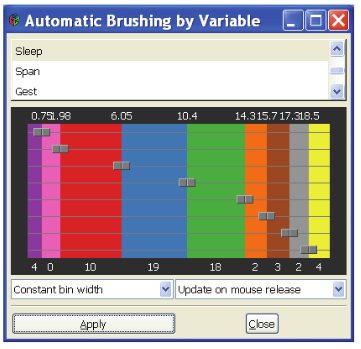
\includegraphics[width=0.8\columnwidth]{9.png}
    \caption{Bôi màu được chỉnh tự động trong GGobi. Người dùng có thể gán bất cứ chiều dữ liệu nào để điều chỉnh màu sắc và có thể điều chỉnh khoảng màu được sử dụng.}
\end{figure}

Một trong những công cụ mạnh mẽ nhất trong ứng dụng GGobi là khả năng tạo và xem “grand tours” của dữ liệu, sử dụng một đường qua không gian chiếu để trình chiếu dữ liệu ở tất cả các view, hoặc từ các tập con ràng buộc với người dùng ở mỗi view. Người dùng có thể thay đổi tốc độ chuyển động và dừng lại để kiểm tra các đặc trưng mong muốn, cũng như xem các tham số mà tạo ra các view.

Nhiều công cụ khác đã được thêm vào GGobi trong thời gian dài, bao gồm liên kết với các gói thư viện thống kê bằng ngôn ngữ R, hỗ trợ cho vài phương pháp vẽ đồ thị (xem hình 15.9), các phương pháp để xử lý dữ liệu bị thiếu, các phương pháp giảm chiều dữ liệu như PCA và MDS.

\begin{figure}[!ht] % [!ht] forces the figure to be output where it is defined in the code (it suppresses floating)
    \centering
    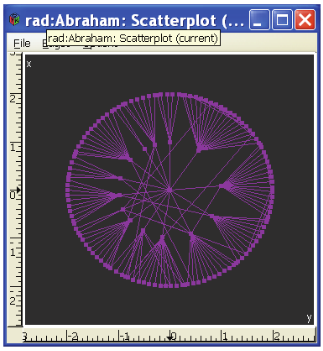
\includegraphics[width=0.7\columnwidth]{10.png}
    \caption{Ví dụ về vẽ đồ thị trong GGobi. Trình bày theo hình tỏa tròn là một trong vài cách trình bày được hỗ trợ.}
\end{figure}

Phần mềm có thể chạy trên Windows, Mac và Linux. Code, tệp thực thi, tài liệu và các hỗ trợ khác có thể được tìm thấy trên website của GGobi.

Các phần mềm khác dùng cho phân tích và đồ thị thống kê bao gồm SPSS (trả phí), và SAS (trả phí), và những phần mềm này có nhiều chức năng hơn là chỉ trực quan hóa thống kê.


%------------------------------------------------

\subsection{Không gian - Thời gian}
Macrofocus đã phát triển một số công cụ tương tác mạnh mẽ cho khai phá dữ liệu và thông tin một cách trực quan. Một trong số đó là InfoScope, liên kết các view địa lý với một vài các biểu diễn bằng hình ảnh hoặc chữ. Một ví dụ của màn hình chính của InfoScope được biểu diễn ở 0. Trong ví dụ này, thông tin từ Liên hợp quốc về phát triển con người có thể được khai phá bằng nhiều cách khác nhau.

\begin{figure}[!ht] % [!ht] forces the figure to be output where it is defined in the code (it suppresses floating)
    \centering
    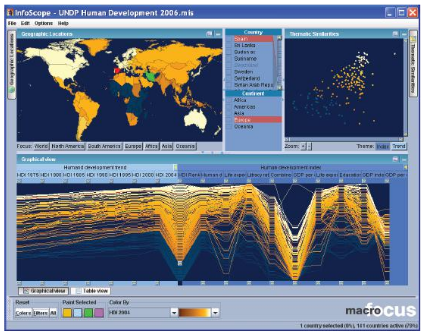
\includegraphics[width=0.8\columnwidth]{11.png}
    \caption{Một ví dụ về màn hình của InfoScope.}
\end{figure}

View địa lý (1) chỉ ra view toàn cầu hoặc view địa phương của các thành phần địa lý trong tập dữ liêu. Một ống kính mắt cá được sử dụng để thu phóng giữ ngữ cảnh bằng cách giữ chuột.

\begin{figure}[!ht] % [!ht] forces the figure to be output where it is defined in the code (it suppresses floating)
    \centering
    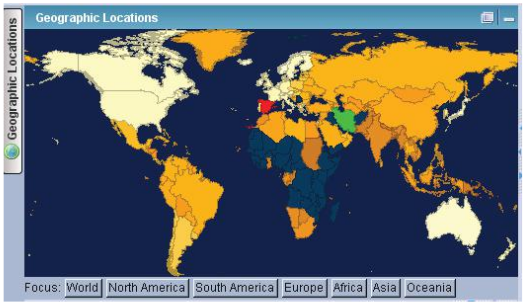
\includegraphics[width=0.8\columnwidth]{12.png}
    \caption{View địa lý trong InfoScope: người dùng có thể lựa chọn các nút cho trước hoặc ấn vào vị trí trên bản đồ.}
\end{figure}

View chủ đề (2) trình chiếu các điểm dữ liệu được trình bày dựa trên sự tương tự sử dụng một thuật toán MDS tối ưu.

\begin{figure}[!ht] % [!ht] forces the figure to be output where it is defined in the code (it suppresses floating)
    \centering
    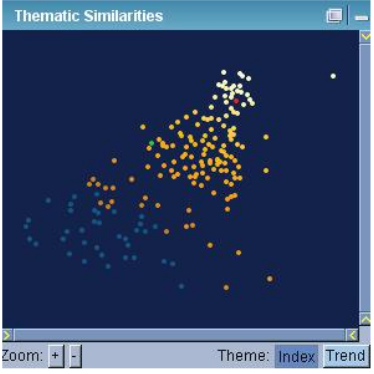
\includegraphics[width=0.5\columnwidth]{13.png}
    \caption{View theo chủ đề trong InfoScope: người dùng có thể lựa chọn từ một số các cách trình bày khác nhau mà biểu diễn mối liên hệ giữa các dữ liệu.}
\end{figure}

View dữ liệu (3) có thể thể hiện dữ liệu hoặc dưới dạng tọa độ song song hoặc bảng biểu.

\begin{figure}[!ht] % [!ht] forces the figure to be output where it is defined in the code (it suppresses floating)
    \centering
    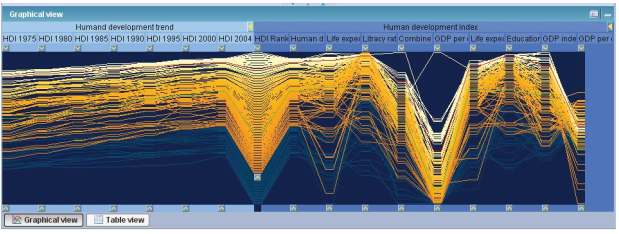
\includegraphics[width=0.8\columnwidth]{14.png}
    \caption{View đồ họa trong InfoScope, với các tọa độ song song để vẽ dữ liệu. Các dữ liệu thấp hơn trên một trong các chiều đã bị lọc đi, kết quả là màu tối cho những dữ liệu này trong các view.}
\end{figure}


Sức mạnh của InfoScope nằm ở liên kết chặt chẽ của nó với các view khác nhau. Bôi màu trong bất cứ view nào sẽ bôi đâm dữ liệu tương ứng trong tất cả các view còn lại. Lên tới 4 loại bút tô có thể được sử dụng để tách biệt từng ghi chép cho hiển thị song song. Dữ liệu có thể dược lọc bằng cách kéo các trình điều khiển ở trên hoặc dưới cùng của mỗi trục tọa độ song song để cho phép người dùng làm mờ đi các giá trị cao hoặc thấp. Màu sắc có thể được liên kết với bất cứ biến dữ liệu nào, vì vậy người dùng có thể dễ dàng chuyển đổi giữa các bản đồ theo chủ đề khác nhau. Di chuột qua các điểm dữ liệu sẽ hiện lên nhãn hoặc giá trị một cách trực quan.

Các hiệu ứng chuyển động cũng được sử dụng hiệu quả trong InfoScope. Các chức năng thu phóng trong mỗi màn hình được thực thi một cách liền mạch, cho phép người dùng dễ dàng theo sát ngữ cảnh. Các chiều dữ liệu trong các tọa độ song song có thể được co lại hoặc dãn ra giúp dễ dàng phân tích. Trong view chủ đề, chuyển đổi giữa các chủ đề khác nhau tạo ra một hiệu ứng liền mạch về sự chuyển động của các điểm dữ liệu, cho phép người dùng tách biệt các mối quan hệ mà bất biến tương đối giữa các chủ đề với các điểm dữ liệu mà khác biệt đáng kể dựa trên chủ đề.

Phần mềm Macrofocus không hẳn là phần mềm miễn phí; công ty phân phối tệp thực thi miễn phí và cho phép người dùng khám phá một số tập dữ liệu mà Macrofocus cung cấp, nhưng để nhập vào dữ liệu của mình, thì người dùng cần phải trả phí qua trang web của công ty.

Trực quan hóa không- thời gian là một thế mạnh của các hệ thống thống tin theo địa lý. Bên cạnh InfoScope, còn có một số phần mềm khác như là GRASS, ArcGIS, và ERDAS IMAGINE.



%----------------------------------------------------------------------------------------
%	SECTION 3
%----------------------------------------------------------------------------------------
\section{Phân tích và trực quan hóa dữ liệu dạng text}
Jigsaw là một công cụ trực quan hóa dữ liệu dạng text được phát triển bởi John Stasko và các cộng cự ở Viện công nghệ Georgia. Hệ thống này khai phá các thực thể (người, nơi chốn, ngày, tiền tệ) và các mối quan hệ giữa chúng. Jigsaw sử dụng một vài view khác nhau để biểu diễn dữ liệu tới người dùng bao gồm lịch, danh sách, đồ thị, biểu đò phân tán, text và các view theo thời gian, như được trình bày ở 4. Mỗi view được biểu diễn như là một cửa sổ riêng biệt mà cập nhật tự động với các kết quả của query khác nhau.


\begin{figure}[!ht] % [!ht] forces the figure to be output where it is defined in the code (it suppresses floating)
    \centering
    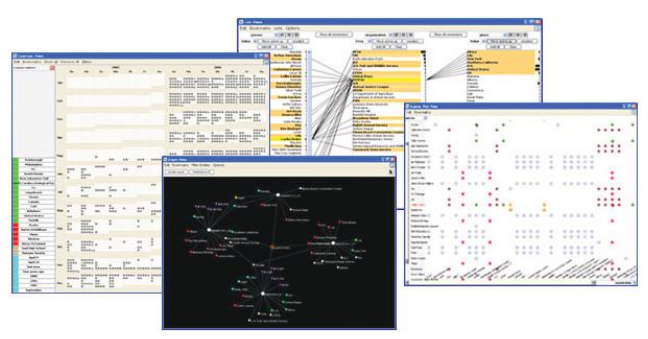
\includegraphics[width=0.8\columnwidth]{15.png}
    \caption{Ví dụ về các view khác nhau trong Jigsaw. Tương ứng là view dạng danh sách, dạng biểu đồ phân tán, đồ thị và theo thời gian.}
\end{figure}

\begin{figure}[!ht] % [!ht] forces the figure to be output where it is defined in the code (it suppresses floating)
    \centering
    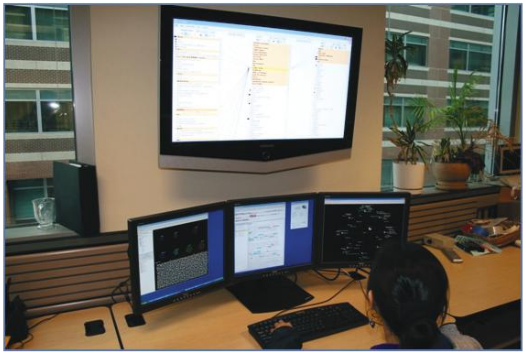
\includegraphics[width=0.8\columnwidth]{16.png}
    \caption{Ví dụ về cấu hình màn hình sử dụng trong Jigsaw. }
\end{figure}

Tất cả các view được liên kết mặc định với nhau, vậy nên thao tác trên một tài liệu hoặc thực thể ở mỗi view sẽ khiến cho các màn hình khác cập nhật tương ứng. Việc cập nhật có thể ddowwjc bật hoặc tắt ở bất cứ màn hình nào để lưu giữ trạng thái của nó. Nó thường hữu ích khi thực sự chứng kiến các view khi chúng cập nhật, để dễ dàng thấy được chúng thay đổi như thế nào. Người dùng có thể thấy việc cần thiết khi sử dụng Jigsaw với 4 hoặc nhiều màn hình hơn, như ở 5., để thu được hết lợi ích của hệ thống.

Công cụ này đặc biệt hữu ích trong khai phá dữ liệu liên quan tới một tập lớn các dữ liệu và thông tin. Các ứng dụng của nó bao gồm tình báo quân sự, thi hành luật pháp, báo chí, hoặc các lĩnh vực tương đương. Cũng quan trọng khi chỉ ra rằng trong khi công cụ này có thể giúp phân tích trên một số lượng lớn tài liệu, các thực thể và mối quạn hệ giữa chúng, nó không thể thay thế được việc thực sự đọc các tài liệu này. Ví dụ, nó có thể giúp một nhà phân tích xác định tài liệu nào là quan trọng và cần được đọc, giúp tiết kiệm thời gian thay vì đọc toàn bộ tài liệu, điều mà khó khả thi.

%----------------------------------------------------------------------------------------
%	SECTION 4
%----------------------------------------------------------------------------------------
\section{Hệ thống trực quan hóa tích hợp hiện đại}
Tableau là một gói phần mềm thương mại được phát triển đầu tiên bởi Pat Hanrahan và học trò của ông tại Standford. Nó được thiết kế với nhiều tương tác hiện đại để hỗ trợ việc phân tích dữ liệu. Tableau cho phép người dùng nhập vào dữ liệu dưới nhiều định dạng khác nhau. Nó cung cấp các trực quan hóa tiêu chuẩn như đồ thị, biểu đồ phân tán, biểu đồ cột, biểu đồ tròn cũng như bản đồ. Tableau có thể nhận dạng các loại dữ liệu dạng địa lý và tự động xử lí các bước đầu tiên trong quá trình tạo trực quan hóa. Nó cũng hỗ trợ xuất các trực quan hóa bản trình bày có chú thích ở định dạng PDF và cung cấp các bảng điều khiển có tính tương tác mà tự động cập nhật từ các nguồn dữ liệu, cũng như công cụ xuất bản web.

Hình 16 hiển thị bản đồ với dữ liệu được hợp nhất: hình vẽ biểu diễn sản xuất mỏ khí thay đổi từ 2004 đến 2005, và đường đi của bão Rita và Katrina được tô màu theo cường độ của chúng. Bão Rita gây ra nhiều thiệt hại hơn và đối xứng hơn trên đường đi của nó, trong khi thiệt hại của Katrina nhiều hơn ở bên phải của nó, phía nước dâng. Lưu ý hỗ trợ trực quan hóa bản trình bày (chú thích, văn bản, chú thích).

\begin{figure}[!ht]
    \centering
    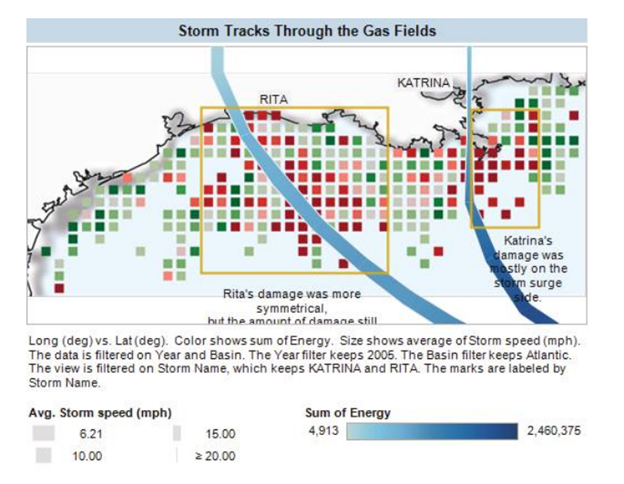
\includegraphics[width=0.8\columnwidth]{15.16}
    \caption{Một ví dụ về các màn hình và bảng được liên kết trong Tableau với các đường dẫn được tô màu theo cường độ bão. Đồ thị biểu diễn nhằm hướng sự chú ý vào vấn đề giao diện và nhận thức. }
\end{figure}
%----------------------------------------------------------------------------------------
%	SECTION 5
%----------------------------------------------------------------------------------------
\section{Các công cụ trực quan hóa dữ liệu}
\subsection{Prefuse}
Prefuse là một công cụ để xây dựng những ứng dụng trực quan hóa. Nó bao gồm 2 thành phần, một phần sử dụng Java và các thành phần còn lại được viết bằng Action-Script. Trước hết nó cung cấp một bộ các giao diện và lớp Java để hỗ trợ lập trình viên tạo những ứng dụng trực quan hóa một cách độc lập hoặc dựa trên web (Java applet). Sau đó, Pressure Flare cho phép người dùng có thể tạo trực quan hóa và hoạt ảnh cho Adobe Flash Player. Prefuse Flare là một thành phần tương đối mới, có phiên bản alpha được phát hành vào tháng 10 năm 2007, trong khi đó bộ công cụ Java-based đầu tiên được phát hành tháng 5 năm 2006. (Prefuse được tích hợp sẵn trong trang web của nó). Prefuse có thể hỗ trợ nhiều cấu trúc dữ liệu, trực quan hóa và những kĩ thuật tương tác như sau:

\begin{itemize}
    \item cấu trúc dữ liệu bảng, đồ thị, và cây
    \item mã hóa bố cục, màu sắc, kích thước và hình dạng khác nhau, biến dạng và hoạt ảnh
    \item các hoạt động tương tác, thao tác trực tiếp thông thường
    \item xem các phép biến đổi, bao gồm xoay và thu phóng;
    \item truy vấn động để lọc tương tác
    \item tích hợp tìm kiếm văn bản
    \item một công cụ mô phỏng lực lượng vật lý cho bố cục động và hình ảnh động
    \item nhiều chế độ xem, bao gồm các lượt hiển thị “tổng quan+chi tiết” và “nhiều phần nhỏ”
    \item một ngôn ngữ biểu thức giống như SQL được tích hợp sẵn để viết các truy vấn
    \item khả năng đưa ra các truy vấn SQL tới cơ sở dữ liệu và ánh xạ các kết quả truy vấn vào các cấu trúc dữ liệu Prefuse
    \item khả năng tạo các thành phần xử lý, tương tác và hiển thị tùy chỉnh

\end{itemize}

Cấu trúc của bộ công cụ Prefuse dựa trên mô hình tham chiếu trực quan hóa thông tin được đề xuất bởi Ed Chi [72]. Mô hình này chia quá trình trực quan hóa thông tin thành nhiều bước riêng biệt. Prefuse đã Prefuse thực thi các bước này như hình bên dưới:

\begin{itemize}
    \item Các phép biến đổi dữ liệu: Các phép biến đổi dữ liệu. Dữ liệu thô được chuyển đổi để xây dựng các bảng dữ liệu, là biểu diễn bên trong của dữ liệu. Lưu ý rằng các bảng dữ liệu có thể cũng đại diện cho dữ liệu mạng hoặc cây, cũng như dữ liệu đa biến, bất chấp tên gọi. Prefuse có thể xử lý nhiều định dạng tệp, chẳng hạn như tệp CSV (giá trị được phân tách bằng dấu phẩy), tệp được phân cách bằng tab, GraphML và TreeML. GraphML và TreeML là hai loại định dạng tệp XML để biểu thị dữ liệu cấu trúc biểu đồ và cây.
    \item Ánh xạ trực quan: Bước này nhằm tạo ra một trừu tượng trực quan, một mô hình dữ liệu bao gồm các đặc điểm trực quan như bố cục không gian, màu sắc, kích thước và hình dạng.
          Prefuse cung cấp khả năng lọc, bố cục, màu sắc, hình dạng và gán kích thước, biến dạng và hoạt ảnh để xây dựng các hình ảnh trừu tượng.

    \item Biến đổi thị giác: Bước này thực hiện kết xuất và tạo các chế độ xem cuối cùng. Một bản tóm tắt trực quan có thể tương ứng với nhiều chế độ xem để hỗ trợ xoay, thu phóng và hiển thị “small multiple”.
\end{itemize}

Dưới đây là vài gói và lớp quan trọng trong công cụ Java-Based Prefuse:

\begin{itemize}

    \item Gói dữ liệu và nhập/xuất dữ liệu (Packages data and data I/O): định nghĩa cấu trúc dữ liệu dạng bảng, cây,đồ thị và đọc hoặc ghi tệp vật lí ở nhiều định dạng khác nhau
    \item Lớp trực quan hóa (Class visualization): tạo ra sự trừu tượng trực quan thông qua việc them dữ liệu được khởi tạo thông qua lớp VisualItem
    \item Lớp hiển thị (Class display): chịu trách nhiệm phần hiển thị cuối cùng
    \item Gói điều khiển (Package controls): cung cấp một số lớp để xử lý các thao tác của chuột và bàn phím trên màn hình giúp các nhà phát triển dễ dàng thao tác
\end{itemize}

Một số hình ảnh từ gói demo Prefuse hoặc các ứng dụng được phát triển bằng Prefuse được hiển thị bên dưới để truyền đạt một số sức mạnh của công cụ.

\begin{figure}[!ht]
    \centering
    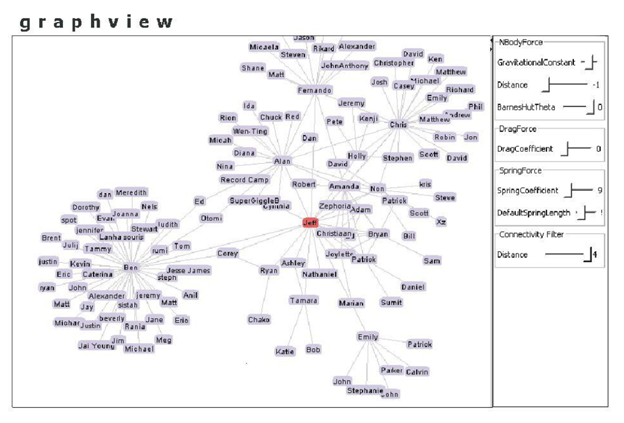
\includegraphics[width=0.65\columnwidth]{15.17}
    \caption{Một ví dụ về đồ thị được tạo bởi Prefuse}
\end{figure}

Hình 17 cho thấy một bộ dữ liệu nhân tạo để truyền tải các mối quan hệ mạng giữa những người khác nhau. Người dùng có thể sử dụng bảng điều khiển ở phía bên phải để điều chỉnh các thông số trực quan cho các nhiệm vụ khám phá khác nhau. Một ví dụ khác là Núi dữ liệu (xem Hình 18), hiển thị hình thu nhỏ cho một số đối tượng. Người dùng có thể kéo và thả các hình thu nhỏ này để quản lý các đối tượng một cách trực quan.

\begin{figure}[!ht]
    \centering
    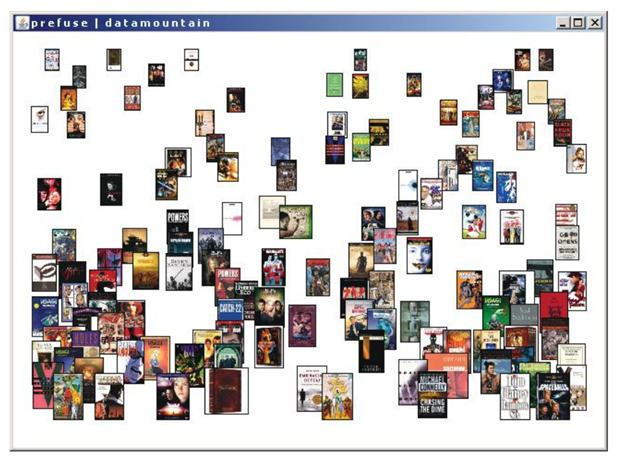
\includegraphics[width=0.65\columnwidth]{15.18}
    \caption{Một ví dụ về đồ thị được tạo bởi Prefuse}
\end{figure}

\begin{figure}[!ht]
    \centering
    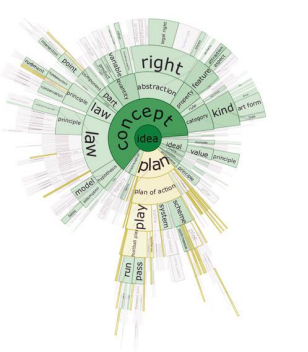
\includegraphics[width=0.6\columnwidth]{15.19}
    \caption{Kiểm tra từ khóa của tài liệu và mối quan hệ của chúng bằng Prefuse}
\end{figure}

DocuBurst là một ứng dụng được phát triển dựa trên Prefuse [82]. Chúng tôi trình bày nó để cho thấy khả năng mở rộng của Prefuse trong việc phát triển các loại ứng dụng trực quan hóa thông tin khác nhau. Hình 19 sử dụng một cây xuyên tâm, lấp đầy không gian để biểu diễn mối quan hệ hyponymy (IS-A) giữa các từ khóa trong tài liệu. Ở cùng cấp độ, độ rộng góc của một từ tỷ lệ thuận với số lần xuất hiện của nó trong tài liệu này. Đồng thời, các nút có viền vàng là kết quả truy vấn cho các từ khóa có cách viết bắt đầu bằng “pl”.

\subsection{Công cụ Visualization}
Công cụ Visualization(VTK) là một công cụ mã nguồn mở dùng để xây dựng trực quan hóa 3D bao gồm đồ họa máy tính, mô hình, ảnh và cả trực quan hóa khoa học và thông tin. Nó cung cấp một số công cụ UI, tiện ích tương tác, hỗ trợ chú thích và thậm chí hỗ trợ tính toán song song. Nó được viết bởi C++, nhưng có sẵn một số trình bao bọc. \\
VTK tuân thủ các quy trình trực quan hóa (và đồ họa) cổ điển. Nó dựa trên mô hình luồng dữ liệu, giống với OpenDX và AVS. Các mô-đun được kết nối vào một mạng và mỗi mô-đun thực hiện các phép biến đổi trên dữ liệu khi nó truyền qua mạng. Các bộ dữ liệu cơ bản là dữ liệu đa giác và các điểm có cấu trúc, cũng như cả lưới có cấu trúc và không có cấu trúc. Chúng đại diện cho các đỉnh, đường, đa giác và dải tam giác (các nguyên tắc cơ bản được hỗ trợ bởi phần cứng đồ họa của những năm 1990), hình ảnh 2D và 3D dưới dạng các điểm có cấu trúc và lưới để phân tích phần tử hữu hạn.\\
Phong cách lập trình tương tự như OpenGL. Bộ công cụ này bao gồm nhiều lớp và là một môi trường cực kỳ phong phú để lập trình, điều chỉnh và phát triển các ứng dụng dựa trên đồ họa 3D. Bộ công cụ mở rộng sức mạnh của OpenGL bằng cách cung cấp các chức năng và điều khiển cấp cao hơn để hiển thị dữ liệu 3D. Trong khi lập trình trong OpenGL yêu cầu xử lý trực tiếp các điểm 3D, thì lập trình với VTK đòi hỏi phải xử lý cấu trúc cấp cao hơn và các điều khiển cấp cao hơn, do đó giúp lập trình viên giảm bớt các chi tiết thấp và giúp phát triển ứng dụng nhanh hơn và ít bị lỗi hơn. Hình 20 hiển thị giao diện VTK làm nổi bật luồng không khí trên máy bay delta bằng cách sử dụng các đường thẳng và Hình 21 hiển thị ảnh chụp cắt lớp vi tính (CT) từ bộ dữ liệu Người phụ nữ có thể nhìn thấy, cũng bao gồm hình ảnh cộng hưởng từ đầy đủ. Một mặt phẳng của da được cắt bằng một quả cầu, để lộ xương bên dưới. Kết xuất số lượng lớn cũng có thể thực hiện được (dữ liệu từ Bill Lorensen, khi làm việc tại General Electric Corporate Research and Development\\
Ví dụ về các ứng dụng được Kitware xây dựng trên VTK bao gồm:

\begin{itemize}
    \item ITK—bộ công cụ mã nguồn mở để đăng ký và phân đoạn hình ảnh
    \item ParaView—một ứng dụng mã nguồn mở để phân tích và trực quan hóa các tập dữ liệu sử dụng tính toán phân tán
    \item VolView—một ứng dụng để trực quan hóa âm lượng tương tác
\end{itemize}

Một bộ công cụ khác để xây dựng trực quan hóa là Bộ công cụ InfoVis

\begin{figure}[!ht]
    \centering
    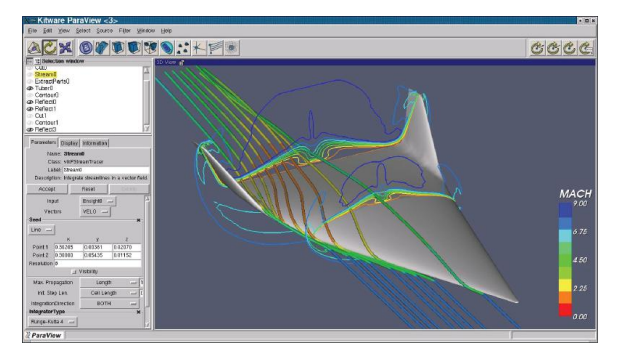
\includegraphics[width=0.8\columnwidth]{15.20}
    \caption{Luồng không khí được mô tả hợp lý trên một máy bay delta. (Hình ảnh từ Kitware, http://www.vtk.org/VTK/project/imagegallery.php.)}
\end{figure}

\begin{figure}[!ht]
    \centering
    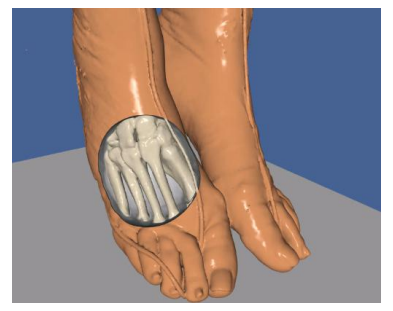
\includegraphics[width=0.8\columnwidth]{15.21}
    \caption{Hình ảnh mô phỏng một phần chân của Người phụ nữ, kết hợp da và xương bên ngoài từ ảnh chụp CT. (Hình ảnh từ Kitware, http://www.vtk.org/VTK/project/ image gallery.php.)}
\end{figure}

\subsection{Weave}

Weave là bộ công cụ trực quan hóa phần mềm hiện đại mã nguồn mở  dựa trên web, được phát triển bởi Georges Grinstein và các sinh viên của ông tại Viện nghiên cứu Trực quan hóa và Nhận thức tại Đại học Massachusetts Lowell với sự tài trợ ban đầu từ Hiệp hội Open Indicators. Weave có thể được sử dụng với nhiều nguồn dữ liệu, cơ sở dữ liệu dựa trên máy chủ, bảng tính hoặc bảng. Nó hoạt động với các nguồn dữ liệu mở như CKAN và data.gov. Nó có sẵn tại http://iWeave.org. Weave cung cấp khả năng hiển thị địa lý linh hoạt trong các trang web (xem Hình 22). Nó hỗ trợ nhiều dạng trực quan hóa khác nhau (bao gồm biểu đồ phân tán, biểu đồ thanh hoặc hình tròn, biểu đồ đường, bản đồ nhiệt, RadViz, tọa độ song song, v.v.) và bản đồ với nhiều hướng dẫn pháp lý (ví dụ: vùng lân cận, vùng điều tra dân số, đô thị, khu vực bỏ phiếu và lưu vực sông). Phần mềm hỗ trợ đồng thời nhiều hình ảnh hóa trong một trang web trình duyệt hoặc trên nhiều trang web. Có một phiên bản máy tính để bàn. Dữ liệu có thể được truy cập thông qua các truy vấn SQL. Có trình chỉnh sửa R và khả năng phân tích nâng cao cho các tập dữ liệu lớn thông qua Parallel R. Weave cũng hoạt động với Stata và các công cụ bên ngoài khác như Cytoscape.

\begin{figure}[!ht]
    \centering
    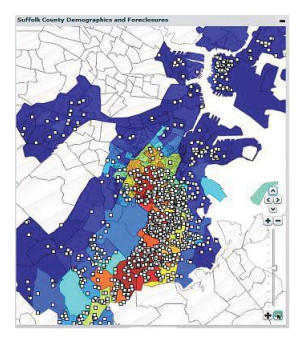
\includegraphics[width=0.8\columnwidth]{15.22}
    \caption{Hình ảnh nhà bị tịch thu (dấu chấm) và tỷ lệ phần trăm dân số da đen (màu sắc) ở khu vực Boston, được tạo bằng công cụ Weave.}
\end{figure}

Mỗi nhà cung cấp dữ liệu (nghĩa là một tổ chức có bộ dữ liệu của riêng họ) thiết lập máy chủ của riêng họ với cài đặt bảo mật được xác định. Sau đó, khách hàng có thể truy cập dữ liệu này trên web từ một ứng dụng web duy nhất—nghĩa là người dùng có thể yêu cầu xem xét cả Boston và Atlanta để so sánh cả hai (trong trường hợp này, nó tải xuống dữ liệu Boston từ máy chủ Boston và dữ liệu Atlanta từ máy chủ Atlanta).
Người dùng có thể mở tập dữ liệu, xem và tương tác với bản đồ hoặc các công cụ trực quan hóa khác, cộng tác với những người dùng khác và xem lại hoặc bắt đầu lại các phiên trước đó. Dữ liệu được tải xuống được lưu vào bộ nhớ cache ở phía máy khách để cung cấp (a) tương tác nhanh hơn sau lần tải xuống đầu tiên và (b) giảm thiểu băng thông giữa máy khách và máy chủ. Có ba công nghệ chính được sử dụng để tạo giao diện máy khách: Adobe Flex, JavaScript và Flex SharedObjects.

Giao diện máy khách bao gồm các công cụ điều hướng tập dữ liệu và trực quan hóa, lịch sử phiên, hỗ trợ kể chuyện, chú thích, cài đặt tùy chọn người dùng và các tính năng cộng tác (bao gồm nhận thức, không gian riêng tư và công cộng, và trò chuyện bằng giọng nói). Chú thích cho phép người dùng thêm nhận xét và diễn giải của riêng họ vào các công cụ trực quan và trạng thái mà họ tạo. Sở thích của người dùng là liên tục; bất cứ khi nào người dùng đăng nhập, các tùy chọn sẽ được khôi phục. Hình 22 cho thấy một bản đồ ví dụ. Các trang web Weave khác bao gồm Metrobostondatacommon.org và Ridatahub.org.


%----------------------------------------------------------------------------------------
%	SECTION 6
%----------------------------------------------------------------------------------------
\section{Thư viện}
\subsection{D3.js}
D3, Data Driven Documents (xem hình 23) ban đầu được phát triển bởi Bostock, Heer và Ogievetsky của nhóm Stanford Visualization như một phần tiếp theo của Protovis và là một khung cung cấp cho việc tạo và kiểm soát các dạng tương tác khi chạy trên web. D3 hỗ trợ một kiểu mã chức năng. D3 làm việc tốt trên những trình duyệt web hiện đại và thư viện lõi của nó có các yêu cầu tối thiểu, cụ thể là các tiêu chuẩn JavaScript và W3C DOM API, Đồ họa vectơ có thể mở rộng (SVG), HTML5 và Cascading Style Sheets (CSS). Điều này cho phép D3 nhúng các hình ảnh động và tương tác trong một trang HTML và áp dụng các chuyển đổi theo hướng dữ liệu cho tài liệu. Mục tiêu chính của nó là thao tác với đối tượng tài liệu đồng thời cải thiện tính tương thích và khả năng sử dụng lại của thư viện.

Do đó, thư viện JavaScript D3.js cho phép lập trình viên sử dụng các hàm JavaScript dựng sẵn để chọn các phần tử, tạo đối tượng SVG, tạo kiểu cho chúng hoặc thêm hiệu ứng chuyển tiếp, hiệu ứng động… Các đối tượng này cũng có thể được tạo kiểu rộng rãi bằng CSS.

Các tập dữ liệu có thể được liên kết với các đối tượng SVG bằng cách sử dụng các hàm D3 đơn giản để tạo các hình ảnh trực quan khác nhau. Dữ liệu có thể ở nhiều định dạng khác nhau, phổ biến nhất là JSON nhưng cũng như hầu hết các bộ công cụ khác, các hàm JavaScript có thể được viết để đọc các định dạng dữ liệu khác và thực hiện chức năng mở rộng.

\begin{figure}[!ht]
    \centering
    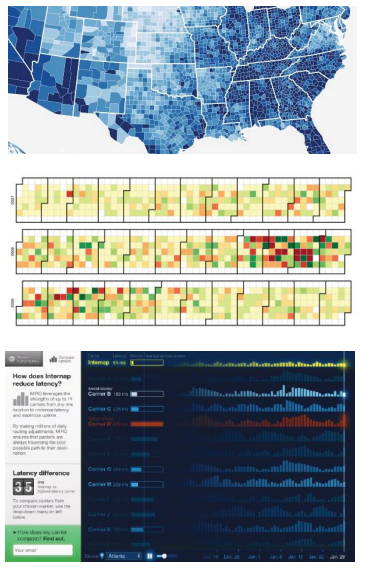
\includegraphics[width=0.8\columnwidth]{15.23}
    \caption{Vài ví dụ về trực quan hóa dữ liệu dùng D3JS}
\end{figure}

\subsection{QGIS}
QGIS là một hệ thống thông tin địa lý nguồn mở (GIS) và là một dự án chính thức của tổ chức Open Source Geospatial Foundation (OSGeo). Nó chạy trên Linux, Unix, Mac OSX, Windows và Android và hỗ trợ nhiều các định dạng và chức năng của vector, raster, và cơ sở dữ liệu. Nó hỗ trợ tạo bản đồ trên web (xem Hình 24).

\begin{figure}[!ht]
    \centering
    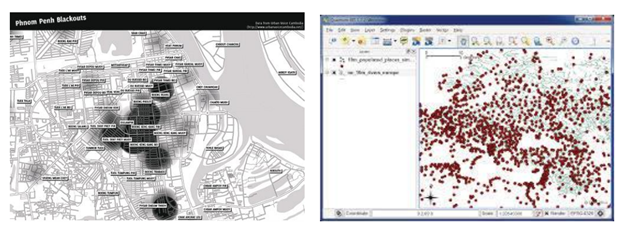
\includegraphics[width=1\columnwidth]{15.24}
    \caption{Vài ví dụ về trực quan hóa dữ liệu dùng QGIS}
\end{figure}

\subsection{Google Maps}
Google Maps là một ứng dụng web cung cấp nhiều dịch vụ liên quan đến bản đồ, ví dụ như chỉ đường cho xe ô tô, người đi bộ hoặc phương tiện giao thông công cộng, tìm chuyến đi, chuyển tuyến và thông tin giao thông, chế độ xem đường phố hoặc từ trên không, tất cả đều có khả năng tương tác trên bản đồ phân lớp (xem Hình 25). Người dùng có thể tương tác với các bản đồ được hiển thị bằng cách thêm các lớp, chẳng hạn như giao thông và chỉ đường, cũng như hiển thị nhiều loại bản đồ khác nhau. Mặc dù Google Maps được sử dụng miễn phí nhưng đây là ứng dụng độc quyền và các chỉnh sửa hoặc mục đích sử dụng khác có thể yêu cầu một số hình thức đăng nhập (ví dụ: hồ sơ hoặc giấy phép).

Google Maps cung cấp nhiều tính năng hỗ trợ việc xây dựng ứng dụng rất phong phú và thú vị. Ví dụ: hướng dẫn di chuyển bằng giọng nói, đề xuất nhà hàng dựa trên vị trí hiện tại của bạn, xác định địa danh hoặc lịch trình của phương tiện giao thông công cộng đến các địa danh đó. Điều này làm cho Google Maps rất giống với thư viện mashup, theo đó người dùng có thể kết hợp Google Maps với các dữ liệu và ứng dụng khác.

\begin{figure}[!ht]
    \centering
    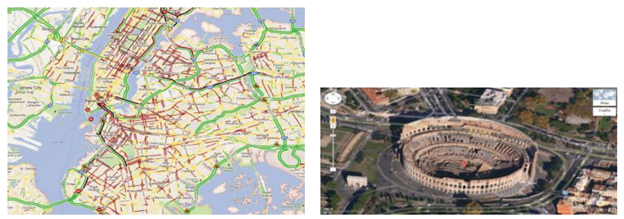
\includegraphics[width=1\columnwidth]{15.25}
    \caption{Ví dụ về trực quan hóa dữ liệu dùng Google Maps}
\end{figure}

\subsection{Circos}
Circos là một hình ảnh đồ thị xuyên tâm được phát triển bởi Martin Krzywunski tại Trung tâm Michael Smith Genomic Sciences Center của Canada (xem Hình 26). Mặc dù công dụng ban đầu của nó là hiển thị dữ liệu bộ gen, nhưng sau đó nó cũng đã được áp dụng cho nhiều lĩnh vực ứng dụng khác. Tuy nhiên thế mạnh của nó vẫn là trong sinh học.

Nó hiển thị các mối quan hệ giữa tất cả các bản ghi trong một vòng kết nối. Các cung trong biểu đồ hiển thị các kết nối với các điểm khác và do đó, Circos là hình ảnh trực quan của các biểu đồ trong một miền hình tròn. Với thứ tự thích hợp như trong RadViz, nó giúp chúng ta có thể phân biệt được các nhóm.

\begin{figure}[!ht]
    \centering
    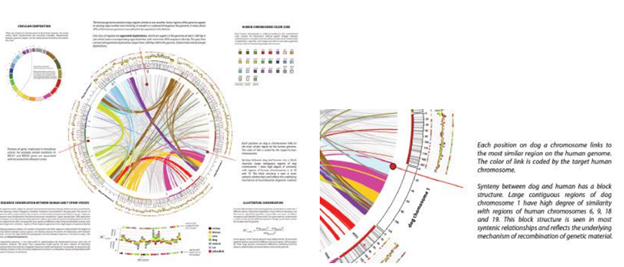
\includegraphics[width=1\columnwidth]{15.26}
    \caption{Trực quan hóa Circos với phần được phóng to (từ http://circos.ca/guide/genomic/img/circos-conservation.png).}
\end{figure}

\section{Tài liệu liên quan}
Một số cuốn sách về trực quan hóa chứa các mô tả về các hệ thống đang được sử dụng hiện nay. Một số, chẳng hạn như [83, 366, 408], mô tả một gói duy nhất, trong khi một số tài liệu khác, bao gồm [390, 405], có số liệu và mô tả từ nhiều hệ thống.

\section{Bài tập}
1. Kiểm tra chức năng của hai công cụ trực quan tập trung vào cùng một loại dữ liệu, một miền thương mại và một miền công cộng. Bạn sẽ mô tả những điểm tương đồng và khác biệt chính của chúng như thế nào? Trong những điều kiện nào và vì những lý do gì, bạn sẽ chọn sử dụng cái này hơn cái kia (tất nhiên bao gồm cả chi phí)?

2. Tìm kiếm trên web một công cụ trực quan không được đề cập trong chương này. Viết một bản tóm tắt về hệ thống theo phong cách tương tự như những gì được trình bày ở đây. Bao gồm các liên kết đến các trang web thích hợp và các bài báo đã xuất bản.

Nếu bạn muốn, hãy gửi tác phẩm kết quả đến trang web sách. Những bài viết chính xác và tốt sẽ được đăng cho các độc giả cùng đọc.

3. Chọn một trong các hệ thống trực quan được mô tả trong chương này và mô tả một số ứng dụng có thể có của hệ thống. Khuyến khích sử dụng web để xác định các phiên bản của ứng dụng “thực”, cũng như sử dụng trí tưởng tượng của mình.

\section{Một số đề tài }
1. Tải xuống, cài đặt và kiểm tra ít nhất một trong các hệ thống trực quan hóa được mô tả trong chương này. Bạn nên cố gắng nhập tập dữ liệu vào hệ thống từ đầu, thay vì sử dụng tập dữ liệu được cung cấp cùng với hệ thống.s

2. Tải xuống và cài đặt một trong các bộ công cụ được mô tả trong chương này. Thực hiện theo các hướng dẫn để tạo một ứng dụng đơn giản, chẳng hạn như biểu đồ phân tán hoặc biểu đồ đường, bằng cách sử dụng bộ công cụ. Viết tóm tắt về trải nghiệm của bạn, bao gồm độ khó/dễ khi tạo ứng dụng và mức độ hài lòng của bạn với kết quả.

\end{document}